\begin{activite}[De nouveaux nombres]

\begin{partie}[1\up{ère} approche]
 \begin{enumerate}
  \item Trace une demi-droite graduée d'origine le point $O$ en prenant le centimètre comme unité. Place les points $A(3)$, $B(4)$ et $D(9)$.
  \item Construis le point $C$ tel que $A$ soit le milieu du segment $[BC]$. Quelle est l'abscisse du point $C$ ?
  \item On veut placer le point $E$ tel que $A$ soit le milieu du segment $[DE]$. Que constates-tu ? Comment compléter cette graduation pour résoudre complètement ce problème ? Quelle est alors l'abscisse du point $E$ ?
  \end{enumerate}
\end{partie}

\begin{partie}[2\up{ème} approche]
 \begin{minipage}[t]{0.40\linewidth}
Ce matin, il faisait très froid. La température a augmenté de \textcolor{H1}{$5^\circ$C}, il fait maintenant $3^\circ$C.
 \begin{itemize}
  \item Pour trouver la température de ce matin, nous allons tester différentes valeurs. Recopie puis complète le tableau ci-contre :
  \end{itemize}
  \end{minipage} \hfill%
  \begin{minipage}[t]{0.56\linewidth}
  \centering
  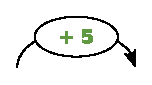
\includegraphics[width=1.9cm]{5}
  
  \begin{tabularx}{0.8\linewidth}{|X|X|}
   \hline
   \rowcolor{J2} Température du matin & Température actuelle \\\hline
   \rowcolor{J2} 5 & \\\hline
   \rowcolor{J2} 3 & \\\hline
   \rowcolor{J2} 1 & \\\hline
   \rowcolor{J2} 0 & \\\hline
   \end{tabularx}
   \end{minipage} \\
   
  \begin{itemize}
  \item Les différentes valeurs testées répondent-elles au problème ? En conséquence, la température du matin peut-elle être supérieure à 0 ?
  \item Quelle était alors la température ce matin ?
  \end{itemize}
\end{partie}

\begin{partie}[Utilisation de ces nouveaux nombres]
Dans quelles circonstances de la vie quotidienne as-tu rencontré des nombres possédant un signe $+$ ou $-$ ? Donne des exemples en histoire, en physique ou dans d'autres domaines. 
\end{partie}

\end{activite}

%%%%%%%%%%%%%%%%%%%%%%%%%%%%%%%%%%%%%%%%%%%%%%%%%%%%%%%%%%%%%%%%%%%%%%

\begin{activite}[Opposés ?]

\begin{enumerate}
 \item Trace une droite graduée d'origine $O$ en prenant le centimètre comme unité.
 \item Place les points $A$ et $C$ d'abscisses respectives $+ 3$ et $- 6$.
 \item Place :
 \begin{itemize}
  \item Le point $B$ tel que $O$ soit le milieu du segment $[AB]$ ;
  \item Le point $D$ tel que $O$ soit le milieu du segment $[CD]$.
  \end{itemize}
 \item Reproduis et complète le tableau ci-dessous : \\[1em]
  \begin{tabularx}{\linewidth}{|c|X|X|X|X|}
   \hline
   \rowcolor{J2} Point & A & B & C & D \\\hline
   \rowcolor{J2} Abscisse du point & $+ 3$ & & $- 6$ & \\\hline
   \rowcolor{J2} Distance du point à l'origine $O$ (en centimètres) & & & & \\\hline
   \end{tabularx} \\[1em]
  On dit que : « La \textbf{valeur absolue} d'un nombre relatif correspond à la distance entre l'origine O et le point qui a pour abscisse ce nombre ». 

 \item Donne la valeur absolue des nombres relatifs suivants : $+ 7$ ; $- 4$ ; $- 6,2$ ; $+ 17,8$.
 \item Donne deux nombres différents qui ont la même valeur absolue. Que constates-tu ? Quel adjectif peux-tu utiliser pour qualifier ces deux nombres ?
 \end{enumerate}
 
\end{activite}

%%%%%%%%%%%%%%%%%%%%%%%%%%%%%%%%%%%%%%%%%%%%%%%%%%%%%%%%%%%%%%%%%%%%%%

\begin{activite}[Manque de repères ?]

On a dessiné un repère du plan sur une carte de Suisse. L'origine de ce repère est la ville de Kerns dans le canton d'Obwald, représentée par le point $O$. \scriptsize{(source de la carte de Suisse : Pymouss, Wikipedia)}

\begin{center} \includegraphics[width=13cm]{carteCH} \end{center}
\normalsize{Le professeur propose de chercher les coordonnées de Locarno qui permettent de la situer par rapport au point $O$ dans ce repère. Voici les réponses de trois élèves de la classe :}
\begin{itemize}
 \item Dylan dit : « Les coordonnées de Locarno, c'est $+ 20$ » ;
 \item Julia dit : « Les coordonnées de Locarno sont d'abord $+ 20$ puis $- 34$ » ;
 \item Medhi dit : « Les coordonnées de Locarno sont d'abord $- 34$ puis $+ 20$ ».
 \end{itemize}
 \begin{enumerate}
  \item Dylan a-t-il donné suffisamment d'informations pour repérer la ville de Locarno ? Dans un repère du plan, combien de nombres sont nécessaires pour repérer un point ?
  \item Les réponses de Julia et Medhi manquent de précision. Pourquoi ? Réécris celles-ci afin qu'elles soient complètes. \\[1em]
Pour écrire les coordonnées d'un point, on écrit d'abord le nombre qui se lit sur l'axe horizontal puis le nombre qui se lit sur l'axe vertical, en les mettant entre parenthèses et en les séparant par un point-virgule.
  \item Écris les coordonnées de Genève, Lausanne, Neuchâtel, Zürich, Fribourg et Poschiavo.
  \item Donne le nom des villes dont les coordonnées sont : $(+ 45 ; 0)$ ; $(+ 40 ; + 31)$ ;­ $(- 27 ; + 9)$ et $(- 35 ; - 32)$.
  \item Quand on va d'Ouest en Est, que remarques-tu concernant le premier nombre des coordonnées ? Quand on va du Nord vers le Sud, que remarques-tu concernant le deuxième nombre des coordonnées ?
  \item Fabien donne les coordonnées d'une ville du quart Nord-Est : $(- 13 ; + 32)$. Luciana lui dit qu'il y a forcément une erreur. Pourquoi ? Corrige l'erreur de Fabien et cite la ville dont il voulait parler.
  \end{enumerate}
  
\end{activite}

%%%%%%%%%%%%%%%%%%%%%%%%%%%%%%%%%%%%%%%%%%%%%%%%%%%%%%%%%%%%%%%%%%%%%%

\begin{activite}[Comparaison de nombres relatifs]
Sur l'axe gradué ci-dessous, on a placé les points $A$ à $H$.

\begin{center} 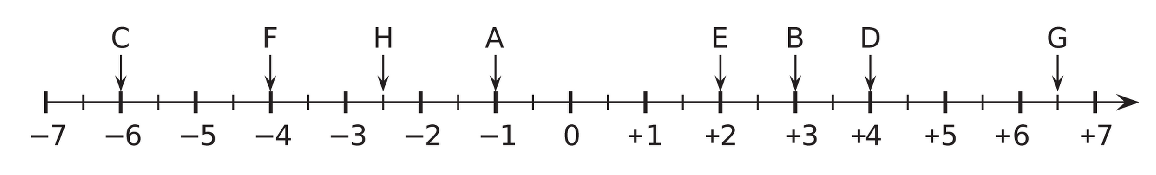
\includegraphics[width=14cm]{axe} \end{center}

 \begin{enumerate}
  \item Lorsqu'on parcourt l'axe gradué de gauche à droite, comment sont rangées les abscisses des points ? Donne les abscisses des points $A$ à $F$ et \textcolor{H1}{$(\geq\ast\ast)$} celles de $G$ et $H$.
  \item En observant l'axe gradué, recopie en remplaçant les .... par $<$ ou $>$ :
   \begin{colitemize}{3}
    \item $- 6 \ldots  \ldots - 1$ ;
    \item $+ 3 \ldots  \ldots - 6$ ;
    \item $+ 4 \ldots  \ldots - 6$ ;
    \item $- 1 \ldots  \ldots + 2$ ;
    \item $+ 2 \ldots  \ldots + 4$ ;
    \item $+ 4 \ldots  \ldots + 3$ ;
    \item $- 1 \ldots  \ldots - 4$ ;
    \item $- 4 \ldots  \ldots - 6$ ;
    \item $- 2,5 \ldots  \ldots + 6,5$.
    \end{colitemize}
  \item Entoure en rouge les cas pour lesquels tu as comparé deux nombres positifs. Observe ces cas et déduis-en une règle qui permet de comparer deux nombres positifs. Tu utiliseras l'expression « valeur absolue » pour rédiger cette règle. 
  \item Entoure en bleu les cas pour lesquels tu as comparé un nombre positif et un nombre négatif. Observe ces cas et déduis-en une règle qui permet de comparer un nombre positif et un nombre négatif.
  \item Entoure en vert les cas pour lesquels tu as comparé deux nombres négatifs. Observe ces cas et déduis-en une règle qui permet de comparer deux nombres négatifs. Tu utiliseras l'expression « distance à zéro » pour rédiger cette règle.
  \end{enumerate}
  
\end{activite}

